The video game industry is a very fast growing business, with hundreds of millions of sales per year. Real time strategy (RTS) games are one of the most sold genre \cite{claypool2005effect}.

RTS games are the basis of many interesting simulations (not only for entertainment). Indeed, such simulations are of great use for researchers and serious games developers. RTS games are used for AI research \cite{buro2004call}, simplified military simulations \cite{buro2003real}, learning \cite{sharma2007transfer}, etc.

Because of these reasons RTS games are the focus of our research. In particular, we focus our research on how serious games developers and researchers develop RTS games.

Building RTS games, and games in general, is difficult because of complex concurrent patterns on heterogeneous entities, within the constraint that the game must run fast. RTS games are developed by mean of either specialized tools or \textit{general purpose tools} (GPT). Specialized tools are used by companies and usually are privately built-in and maintained inside the company itself \cite{buro2005development}. These tools are very expensive to build, so they are typically employed by large studio's (tens of developers). General purpose tools are used by small studio's (roughly up to 10 developers) and are typically open or require licensing to be used. Researchers and serious games developers belong to the small studio category and they use GPT's to implement their research; hence GPT's are the focus of our research.

Among the GPT's we find: Unity3D, Unreal Engine, Game Maker, and ORTS. Unfortunately, such tools are general purpose and thus are not specifically designed with development of RTS games as unique goal. To use GPT's for the building of a specific game genre such as an RTS, since GPT's come with some extension facilities. These extension facilities are called \textit{scripting languages}, which are designed to allow developers to build new behaviors in their tool.

Typically, the scripting language used by a GPL is a \textit{general purpose language} (GPL) such as C\# for Unity3D, C++ for Unreal Engine, etc. Unfortunately, GPL's lack specific domain constructs and functionalities related to games. Such limitations affect performance (due to the lack of domain optimization), maintainability, readability and ultimately expressiveness. This leads to poor management of complexities and thus to high costs \cite{costs_of_gpls}.

With big expenses come missed chances: limited resources in research and in the serious games panorama push developers to reduce the amount of features or the depth of these games. Therefore, the opportunity to make innovations is reduced. 

Here our work comes into play, tools designed around the domain of games, which do not limit developers in terms of expressiveness and keep development costs low, are necessary in order to (\textit{i}) allow innovative projects to see the end of their development process, and (\textit{ii}) provide developers with the right tools to tackle features that, with limited tools, might not be built.

\vspace{0.25cm}
\noindent\fbox{%
	\parbox{\textwidth}{%
		\textbf{Our proposal} is to describe how to implement RTS games, based on some taxonomy of such games, in a way that is reusable, scalable, flexible, and shich can be implemented at high performance. To achieve this we propose a series of implementation strategies within the Casanova 2 language \cite{casanova}, a domain specific language (DSL) for games.
    }%
}

\vspace{0.25cm}
\noindent
Thanks to our approach, RTS's become simpler to build and require less effort. This is all to the advantage of those developers with limited resources that we focus on.


In this paper we discuss the design of RTS's by mean of a case study. We discuss pitfall and difficulties in the making of RTS's and show how are they solved with traditional tools. We introduce our solution a domain language for making games called \textit{Casanova} for the problem of making RTS's. We then evaluate our solution and conclude the paper with the future works. \textbf{(*MISSING REFS TO SECTIONS*)}

\section{Existing approaches}
\begin{figure}[!h]
\centering
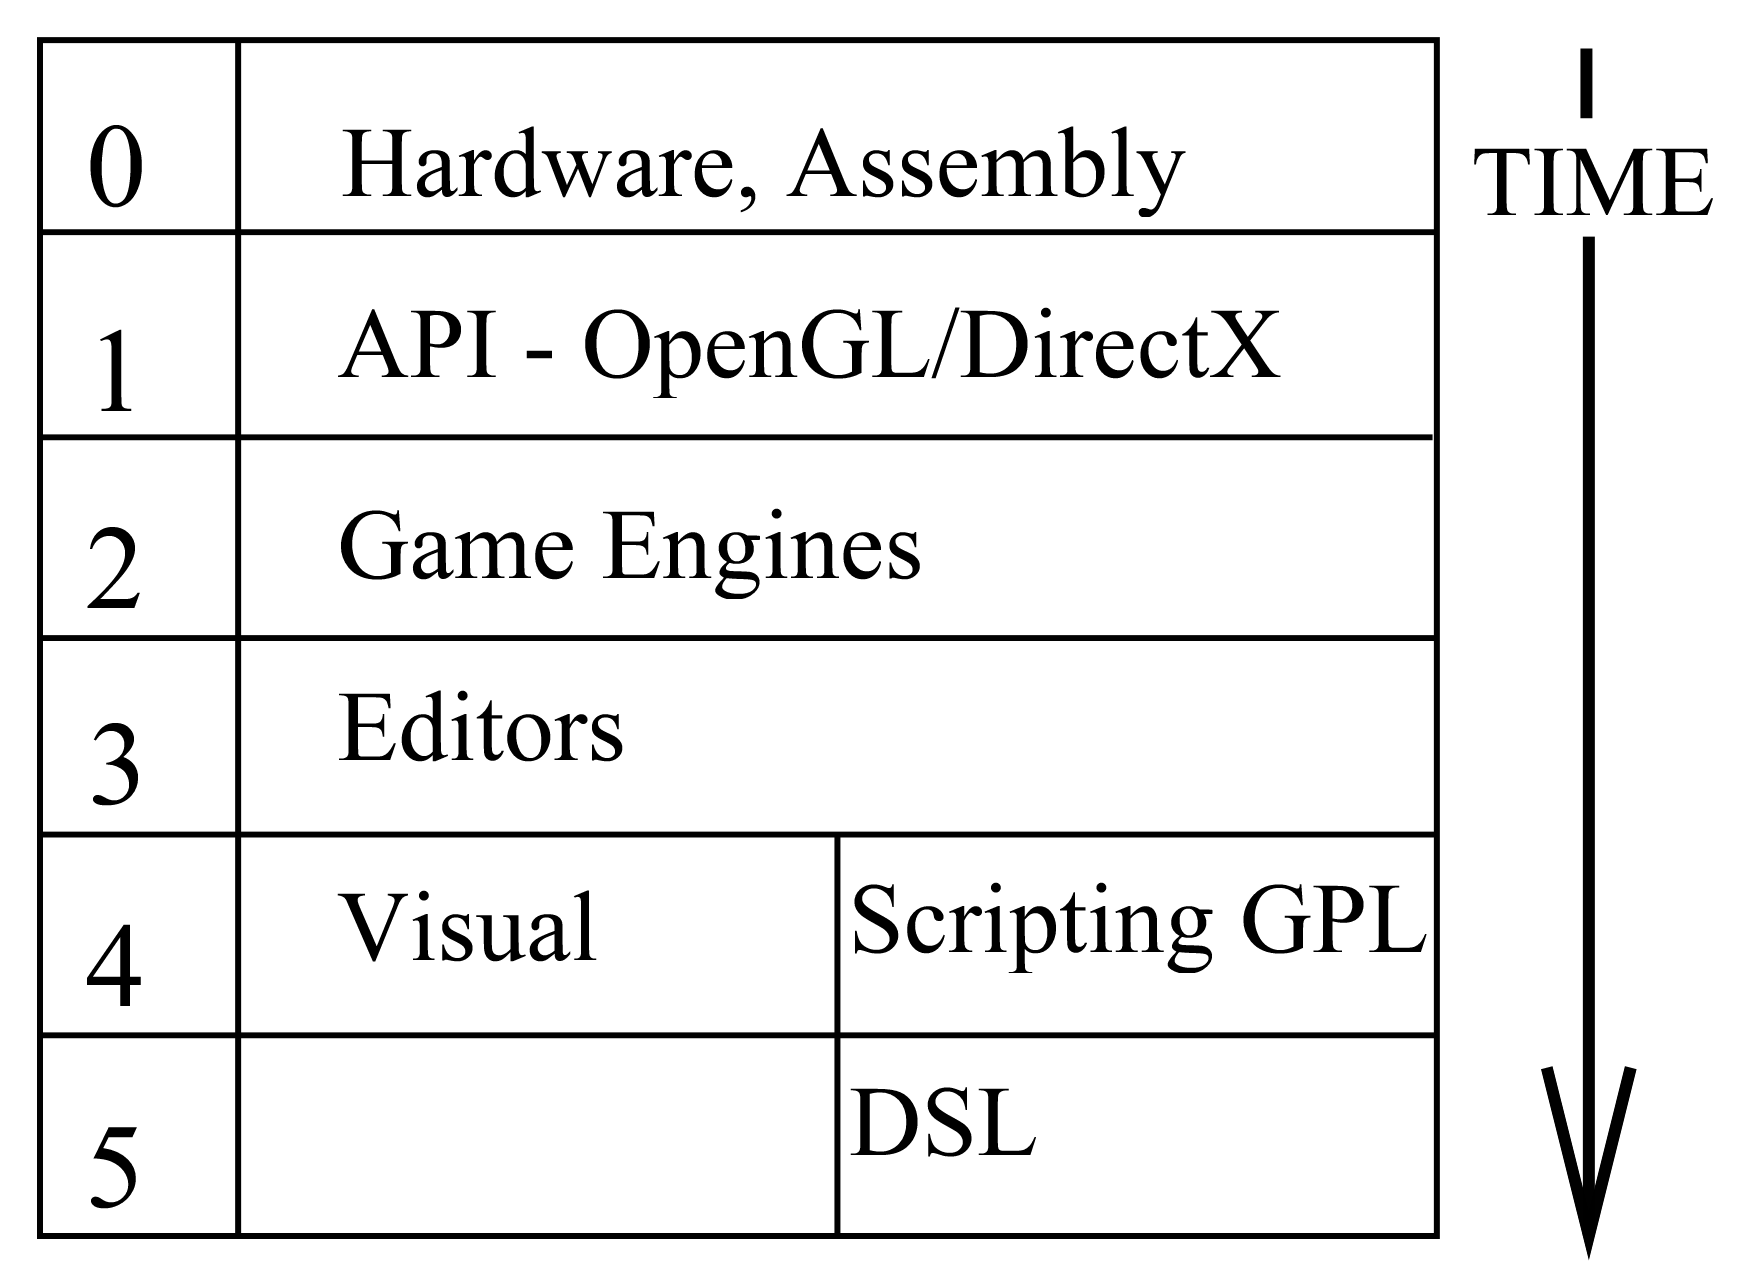
\includegraphics[scale=0.5]{game_development_evolution.png}
\caption{Game development tools evolution}\label{game_dvelopment}
\end{figure}